\documentclass[pdf]{beamer}
\mode<presentation>{}
\usepackage{minted}
\usepackage{tikz}
\usepackage{pgffor} %% gives looping with \foreach
\usepackage[absolute,overlay]{textpos}
\usepackage{lmodern} %% scalable latin characters
\usetikzlibrary{arrows,shapes,backgrounds}
\usepackage{multirow}
\usepackage{listings} %% another package for code related stuff
%\usepackage[fleqn]{amsmath}
\usepackage{fancyvrb}  %% more control over verbatim with /Verbatim

%% stuff for minted
\definecolor{mintedBg}{rgb}{0.95, 0.95, 0.95}
\definecolor{blockBg}{rgb}{0.6, 0.6, 0.95}
\definecolor{rnaColor}{rgb}{0, 0.6, 0}
\definecolor{cdsColor}{rgb}{0, 0.4, 0.4}
\definecolor{rnaPol}{rgb}{0.8,0,0.8}
\definecolor{ribosomeCol}{rgb}{0.5,0.5,0.1}
\definecolor{protColor}{rgb}{0.6,0,0.6}
%% colours for nucleotides:
\definecolor{dACol}{rgb}{0.5, 0.5, 0}
\definecolor{dCCol}{rgb}{0.8, 0, 0}
\definecolor{dGCol}{rgb}{0, 0.8, 0}
\definecolor{dTCol}{rgb}{0, 0, 0.8}

\definecolor{navy}{rgb}{0, 0, 0.6}
\definecolor{pur}{rgb}{0, 0, 0.6}
\definecolor{pyr}{rgb}{0.6, 0, 0.2}

\definecolor{purple1}{rgb}{1.0, 0, 0.6}
\definecolor{purple2}{rgb}{0.8, 0, 0.8}
\definecolor{purple3}{rgb}{0.6, 0, 1.0}
%% define styles for different codes
\newminted{cpp}{linenos, bgcolor=blockBg, fontsize=\footnotesize}
%% then use \begin{cppcode}
\newminted{c}{linenos, bgcolor=mintedBg, fontsize=\footnotesize}
\newminted{perl}{linenos, bgcolor=mintedBg, fontsize=\footnotesize}
\newminted{r}{linenos, bgcolor=mintedBg, fontsize=\tiny}

\setbeamersize{description width=0.57cm}

%% a command to define a subheading
\newcommand\subHeading[1]{
  \par\bigskip {\Large\bfseries#1}\par\smallskip
}

%% I detest indentation in footnotes etc, so try this:
\makeatletter
\renewcommand\@makefntext[1]{\noindent\makebox[0em][r]{\@makefnmark}\tiny#1}
\makeatother
%% the makeatletter and makeatother are required to allow me to
%% to change the macro beginning with an @. (though when I call it
%% I don't use the @ ... 

\setlength\parskip{0.5em}
\setlength\parindent{0ex}

%% to have footnotes without references. This from tex.stackexchange.com
\newcommand\blfootnote[1]{%
  \begingroup  %% this makes it a local redefinition
  \renewcommand\thefootnote{}\footnote{#1}%
  \addtocounter{footnote}{-1}  % this adjusts the footnote counter
  \endgroup
}


%% to draw a pair of genes..
\newcommand{\genePair}[3][]{
        \draw [-,#1] (#2-1,#3) -- (#2+1,#3);
        \draw [-,line width=2, purple1] (#2-0.5,#3) -- (#2+0.5,#3);
        \draw [-,#1] (#2-1,#3-0.5) -- (#2+1,#3-0.5);
        \draw [-,line width=2, purple3] (#2-0.5,#3-0.5) -- (#2+0.5,#3-0.5);  
}

\title{Programming with R}
\subtitle{general isssues}
\author{Martin Jakt}

\begin{document}

\begin{frame}
\titlepage
\end{frame}

\begin{frame}{What is R?}
  \pause
  R is an implementation of S
  \pause
  
  {\small
  \begin{itemize}
  \item An implementation of a statistical programming language (S).
  \item Written by statisticians for statisticians
  \item Makes statistical analysis easy, but general purpose programming difficult.
  \item Usually used in an interactive manner.
  \item Has become the dominant platform for analysis of large scale biological data.
  \end{itemize}
  }
\end{frame}

\begin{frame}{Using R}
  Can be used directly from a console, just by typing stuff into the
  R session without doing anything else. 

  However, it is better to have a record of the commands you used to create
  data members (i.e. variables), so do use some sort of editor to write your code
  into:
  \begin{itemize}
  \item type code into an editor, copy \& paste into R console.\\
  \item RStudio has both editor and console (more elegant choice)
  \end{itemize}

  \textcolor{navy}{\emph{Be aware of the working directory of your session}}. R will by default save
  output files into its working directory, and if you save your session, it will go
  here as well. In RStudio start by defining a new session or open an old one. From
  the console simply \texttt{cd} to your working directory and run R. You can use
  \texttt{getwd} and \texttt{setwd} to find out and change your working directory.

\end{frame}

\begin{frame}{Essential knowledge}
  \begin{itemize}
  \item Data structures (vectors, arrays, lists, matrices, data.frames)
  \item Data types (numeric, logical, character)
  \item Reading writing data (read.table, write.table, readLines, scan)
  \item Loops with for, apply, sapply, tapply
  \item Drawing arbitrary stuff in R
  \item Defining functions
  \item Vectorised operations (eg. rowSums, colSums, colMeans, rowMeans, ifelse)
  \item Classes and functions in R
  \end{itemize}
\end{frame}

\begin{frame}{The source of all wisdom}
  
  \footnotesize All you ever need to know:

  Advanced R \small by Hadley Wickham

  \url{http://adv-r.had.co.nz/Data-structures.html}

\blfootnote{If my information and Hadley's differ, then I'm wrong}
\end{frame}

\begin{frame}{Data structures}

  {\small
  \begin{description}
    \item[vector] A one dimensional ordered list\footnote{but don't call it a
      list; that's something else.!} 
      of values of a single type (numeric, logical or character).
    \item[matrix] A two dimensional vector. All values of the same type; accessed
      by row and column numbers.
    \item[array] An N-dimensional vector. Can have arbitrary numbers of dimensions.
    \item[list] A special kind of vector that can contain values of different types.
      Lists can contain complex objects like
      lists, dataframes as well as custom objects such as those defined by functions.
    \item[dataframe] A list of lists all of the same length. Dataframes are used to store
      tabular data where the type of the column are not all the same (eg, probe identifiers
      or gene names, and expression values).
  \end{description}
}
\end{frame}

\begin{frame}{Data types}
  In R we essentially deal with 4 different types of objects:
  \begin{description}
  \item[numeric] Integers and real numbers (doubles). Numbers are by default read as real
    numbers (continuously variable) but can be forced to integer
    type\footnote{But note that R only has 32 bit integers.}.
  \item[character] Text, strings made up of characters.
  \item[logical] TRUE / FALSE values.
  \item[classes] Objects with some specified structure. Often implemented as named lists.
  \end{description}
  
  R also deals with imaginary and complex numbers, so the above is a little oversimplified.
\end{frame}

\begin{frame}[fragile]{Assignment}
  In R:

  The assignment operator is: \verb|<-|
  \begin{rcode}
    ## assigns the value 10 to a:
    a <- 10;
  \end{rcode}

  Assignment can also be done using \verb|=|
  \begin{rcode}
    ## does the same thing as above
    a = 10;
  \end{rcode}

  But it's better to use \verb|<-| as it is less easy to confuse\footnote{More
    to do with mis-typing than confusing, but whatever..}with the
  equality operator \verb|==| Consider:
  \begin{rcode}
    a <- 10 == 8 ## a <- FALSE
    b = 10 == 10 ## b <- TRUE
  \end{rcode}

\end{frame}

\begin{frame}[fragile]{Numeric types}
  \begin{rcode}
    > a <- 1
    > b <- 3L
    > is.integer(a)
    [1] FALSE
    > is.double(a)
    [1] TRUE
    > is.numeric(a)
    [1] TRUE

    > is.integer(b)
    [1] TRUE
    > is.double(b)
    [1] FALSE
    > is.numeric(b)
    [1] TRUE

    > is.integer(b/2L)
    [1] FALSE

    > is.integer(4L/2L)
    [1] FALSE

    ## coercing values
    > as.integer(5.4)
    [1] 5
    > as.double(4L)
    [1] 4

    ## big numbers can be written using exponential notation
    > 1e6
    [1] 1e+06

    ## or simply using ^ to raise the power
    > 10^6
    [1] 1e+06
    
  \end{rcode}
\end{frame}

\begin{frame}[fragile]{character}
character type

\begin{rcode}
  > a <- "hello"
  > b <- 'world'

  ## " and ' are interchangable in R. But can be used to define
  ## internal quotation marks: eg..
  
  > c <- "the 3' UTR"
  > d <- 'she said, I "do not like that at all"'
  ## use \ to escape internal quotation marks
  > e <- 'she said, "I don\'t like that at all"'
  ## but note that
  > e
  [1] "she said, \"I don't like that at all\""
  
  ## but cat does the right thing
  > cat(e, '\n')
  she said "I don't like that at all"

  ## to combine strings together use paste
  > paste(a, b)
  [1] hello world

  > paste(a, b, sep="|")
  [1] hello|world
\end{rcode}
\end{frame}

\begin{frame}[fragile]{logical}
  \begin{rcode}
    ## c is the concatenate function. It makes a vector
    > a <- c(TRUE, FALSE, TRUE)
    > a
    [1] TRUE FALSE TRUE

    ## you can be lazy as well:
    > a <- c(T, F, T)
    > a
    [1] TRUE FALSE TRUE
    
    ## you can convert other types to logical
    > a <- as.logical(c(0, 3, 1, 2))
    > a
    [1] FALSE, TRUE TRUE TRUE
    
    ## and the other way around
    > as.numeric(a)
    [1] 0 1 1 1
    
    ## and implicitly by calling a function
    > sum(a)
    [1] 3
    
    ## you can also set up logical values using
    ## comparisons
    > c(1 > 0, 0 > 2, 3 == 4)
    [1] TRUE FALSE FALSE

    ## or vectorised comparisons
    > a <- c(0, 1, 2, 4)
    > b <- c(0, 1, 2, 3)
    > a == b
    [1] TRUE TRUE TRUE FALSE
  \end{rcode}
\end{frame}

\begin{frame}[fragile]{Vectors}
  \begin{rcode}
    ## can be created by concatenation:
    > a <- c(1, 2, 3)
    > a
    [1] 1 2 3
    
    ## but note that the type will end up the same
    > c('a', 'b', 'c')  ## OK!
    [1] "a" "b" "c"
    
    > c('a', 2, 'c') ## maybe not what you want
    [1] "a" "2" "c"
   
    ## numeric ranges
    > 1:4
    [1] 1 2 3 4

    ## by the seq command
    > seq(1, 4, by=0.5)
    [1] 1.0 1.5 2.0 2.5 3.0 3.5 4.0

    ## c gives a flat vector
    > c(1:3, c(4, 5, 6), 9:10)
    [1]  1  2  3  4  5  6  9 10

    ## you can also create empty vectors with
    ## the vector() function
    > vector(length=4, mode='logical')
    [1] FALSE FALSE FALSE FALSE
    > vector(length=4, mode='numeric')
    [1] 0 0 0 0
    > vector(length=4)
    [1] FALSE FALSE FALSE FALSE
    > vector(length=4, mode='character')
    [1] "" "" "" ""
  \end{rcode}
\end{frame}

\begin{frame}[fragile]{Vectors (2)}
Accessing elements of a vector

\begin{rcode}
  ## define a vector
  > a <- 2 * 1:10
  > a
  [1]  2  4  6  8 10 12 14 16 18 20

  ## to get a single element use a single number
  > a[4]
  [1] 8

  ## use a vector of indices to get several elements
  > a[3:4]
  [1] 6 8
  
  ## use negative indices to remove one
  > a[-2]
  [1]  2  6  8 10 12 14 16 18 20
  ## or more elements
  > a[-1:-3]
  [1]  8 10 12 14 16 18 20
  
  ## or use a vector of logical values
  > a > 10
  [1] FALSE FALSE FALSE FALSE FALSE  TRUE  TRUE  TRUE  TRUE  TRUE
  > a[ a > 10 ]
  [1] 12 14 16 18 20

  ## All of these can be used to set values as well
  > a[-1] <- 1:9
  > a
  [1] 2 1 2 3 4 5 6 7 8 9
\end{rcode}
\end{frame}

\begin{frame}[fragile]{Matrices}
  
  { \small
  2 dimensional vectors. Defined by number of rows (\texttt{nrow})
  and by number of columns (\texttt{ncol}).

  \begin{verbatim}
Usage:

     matrix(data = NA, nrow = 1, ncol = 1, byrow = FALSE,
            dimnames = NULL)
\end{verbatim}
}
  \begin{rcode}
    ## data is filled by column by default
    > matrix(1:9, ncol=3)
         [,1] [,2] [,3]
    [1,]    1    4    7
    [2,]    2    5    8
    [3,]    3    6    9
    ## but can be by column
    > matrix(1:9, ncol=3, byrow=TRUE)
         [,1] [,2] [,3]
    [1,]    1    2    3
    [2,]    4    5    6
    [3,]    7    8    9

  \end{rcode}
\end{frame}

\begin{frame}[fragile]{Matrices (2)}
  Specifying the data of a matrix

  \begin{rcode}
    ## no need to specify the data
    > matrix(nrow=3, ncol=4)
         [,1] [,2] [,3] [,4]
    [1,]   NA   NA   NA   NA
    [2,]   NA   NA   NA   NA
    [3,]   NA   NA   NA   NA

    ## or with a repeated values
    > matrix(nrow=3, ncol=4, data='A')
        [,1] [,2] [,3] [,4]
    [1,] "A"  "A"  "A"  "A" 
    [2,] "A"  "A"  "A"  "A" 
    [3,] "A"  "A"  "A"  "A" 

    > matrix(nrow=3, ncol=4, data=c('A', 'B'))
        [,1] [,2] [,3] [,4]
    [1,] "A"  "B"  "A"  "B" 
    [2,] "B"  "A"  "B"  "A" 
    [3,] "A"  "B"  "A"  "B" 

  \end{rcode}

\end{frame}

\begin{frame}[fragile]{Matrices (3)}
  Transposition and dimensions

  \begin{rcode}
    ## t() transposes matrices:
    > matrix(1:4, ncol=2)
          [,1] [,2]
    [1,]    1    3
    [2,]    2    4
    > t(matrix(1:4, ncol=2))
         [,1] [,2]
    [1,]    1    2
    [2,]    3    4

    ## to get the dimensions, use dim(), ncol() and nrow()
    > a <- matrix(ncol=4, nrow=50)
    > dim(a)
    [1] 50  4
    > ncol(a)
    [1] 4
    > nrow(a)
    [1] 50
  \end{rcode}
\end{frame}

\begin{frame}[fragile]{Matrices (4)}
  Accessing elements and slices of matrices:

  \begin{rcode}
    # a matrix a
    > a <- matrix(1:9, ncol=3)

    ## to get a single element specify both row
    ## and column
    > a[2,2]
    [1] 5
    
    ## to get a row or colum:
    > a[1,]
    [1] 1 4 7
    > a[,1]
    [1] 1 2 3

    ## or several colums or rows
    > a[1:2,]
         [,1] [,2] [,3]
    [1,]    1    4    7
    [2,]    2    5    8

    ## you can use negative numbers as before
    > a[-1,]
         [,1] [,2] [,3]
    [1,]    2    5    8
    [2,]    3    6    9
    
    ## and logical vectors and so on...
  \end{rcode}
\end{frame}

\begin{frame}[fragile]{Matrices (5)}

  {\small
  \texttt{cbind()} and \texttt{rbind} are like \texttt{c()} but for matrices.
  
  can be used to combine vectors to matrices and matrices
  to matrices:
}
  \begin{rcode}
    ## make a couple of vectors
    > a <- 1:5
    > b <- 11:15
    ## and play around with them:
    > cbind(a,b,b,a)
         a  b  b a
    [1,] 1 11 11 1
    [2,] 2 12 12 2
    [3,] 3 13 13 3
    [4,] 4 14 14 4
    [5,] 5 15 15 5

    > rbind(a,b,a)
      [,1] [,2] [,3] [,4] [,5]
    a    1    2    3    4    5
    b   11   12   13   14   15
    a    1    2    3    4    5

    ## can nest the calls as we like
    > cbind( cbind(a,a), rbind(b,b,b,b,b) )
      a a               
    b 1 1 11 12 13 14 15
    b 2 2 11 12 13 14 15
    b 3 3 11 12 13 14 15
    b 4 4 11 12 13 14 15
    b 5 5 11 12 13 14 15
    
    ### But note that dimensions must be compatible!!!
  \end{rcode}
\end{frame}

\begin{frame}[fragile]{Matrices Warning}
  Extracting a single row converts the value to a vector.
  
  A vector has no dimensions / column number / row number.
  \begin{rcode}
    > a <- matrix(1:12, ncol=4)
    > dim(a)
    [1] 3 4
    > dim(a[1:2,])
    [1] 2 4
    > dim(a[1,])
    NULL
    > ncol(a[1,])
    NULL
    
    ## this can cause troubles when you don't know how many rows
    ## or columns will be extracted

    ## use drop=FALSE to avoid this:
    > dim(a[1,,drop=FALSE])
    [1] 1 4
    > ncol(a[1,,drop=FALSE])
    [1] 4
  \end{rcode}
\end{frame}


\begin{frame}[fragile]{Arrays}
  An array is an N-dimensional vector. A matrix is
  a special case.

  \begin{rcode}
    ## eg a cube:
    > array(1:27, dim=c(3,3,3), dimnames=c('x', 'y', 'z'))
    , , 1

        [,1] [,2] [,3]
   [1,]    1    4    7
   [2,]    2    5    8
   [3,]    3    6    9

   , , 2

        [,1] [,2] [,3]
   [1,]   10   13   16
   [2,]   11   14   17
   [3,]   12   15   18

   , , 3

         [,1] [,2] [,3]
   [1,]   19   22   25
   [2,]   20   23   26
   [3,]   21   24   27
  \end{rcode}

  Arrays are not used so commonly, so we will not cover them further here.
\end{frame}

\begin{frame}[fragile]{Lists}
  
  {\small
  Lists are special vectors that can hold different types of elements,
  including nested lists, matrices and dataframes (see later). This 
  means they can be used to represent more complex data structures like
  trees. But they are rather slow to access, so this is generally not a good idea.
  }

  \begin{rcode}
    ## you can use the list() function to make a list:
    > list( 1, "two", 3, 1:4)
    [[1]]
    [1] 1
    
    [[2]]
    [1] "two"
    
    [[3]]
    [1] 3
    
    [[4]]
    [1] 1 2 3 4
    
    ## the resulting list has 4 elements, the last one which is a vector of numbers.
    
    ## you can also provide names when creating a list
    > list("a"=1:3, "b"=3:1)
    $a
    [1] 1 2 3
    
    $b
    [1] 3 2 1
  \end{rcode}
\end{frame}

\begin{frame}[fragile]{accessing list elements}
  To access the elements making up a list you need to make
  use of a double indexing operator \texttt{[[]]}. 

  \begin{rcode}
    > a <- list(a=1:4, b=4:1)
    > a
    $a
    [1] 1 2 3 4
    
    $b
    [1] 4 3 2 1
    
    ## the first element with single []
    > a[1]
    $a
    [1] 1 2 3 4
    
    ## and with [[]]
    > a[[1]]
    [1] 1 2 3 4

    ## we can also access named elements using the $
    ## operator:
    > a$a
    [1] 1 2 3 4
    > a$b
    [1] 4 3 2 1
    > 
  \end{rcode}
\end{frame}
    
\begin{frame}[fragile]{accessing elements (2)}

  {\small
  What happens when we use \texttt{[]} instead of \texttt{[[]]}?
}
  \begin{rcode}
    ## to see what happens when we use single and double
    ## []
    > is.list(a)
    [1] TRUE
    > is.list(a[1])
    [1] TRUE
    > is.list(a[[1]])
    [1] FALSE
  \end{rcode}
  {\small
  Using the usual \texttt{[]} operator returns a list of length one.
  This kind of makes sense if you think of doing \texttt{a[1:2]}.

  A list is a special type of vector and you can create one using the
  \texttt{vector} command:
  }

  \begin{rcode}
    > vector(mode='list', length=3)
    [[1]]
    NULL
    
    [[2]]
    NULL
    
    [[3]]
    NULL
  \end{rcode}
  {\small
  This is useful when you wish to define the length of the list when you
  define it. Extending a list is an expensive operation that can slow down
  your code a great deal so it is better to avoid doing that.
}
\end{frame}

\begin{frame}[fragile]{dataframes}
  
  {\small
    \begin{itemize}
      \item dataframes can be created with the \texttt{data.frame()} function
        and are returned by by many functions that read data from files
        (eg. \texttt{read.table()}).
      \item They are useful for storing tabular data where rows and columns
        can be of different types. They are implemented as a list of lists
        with columns containing independent lists.
      \item  In general they can be used in a similar manner to matrices, but
        there are some situations where this doesn't work. Functions like
        apply will coerce the dataframe to a matrix, and this can cause problems
        if the dataframe contains data of different types.
      \end{itemize}
  }
\end{frame}

\begin{frame}[fragile]{making dataframes}
  Creating a dataframe from a file:
  \begin{Verbatim}[fontsize=\tiny]
                genotype        tissue                          drug
GSM532993       lean (fa/+)     adipose tissue (epididymal)     control
GSM532994       lean (fa/+)     adipose tissue (epididymal)     control
GSM532995       lean (fa/+)     adipose tissue (epididymal)     control
GSM533011       lean (fa/+)     liver                           control
GSM533012       lean (fa/+)     liver                           control
GSM533013       lean (fa/+)     liver                           control
GSM533029       lean (fa/+)     skeletal muscle (gastrocnemius) control
GSM533030       lean (fa/+)     skeletal muscle (gastrocnemius) control
...
  \end{Verbatim}

  \begin{rcode}
    ## read in data from a file containing sample descriptions:
    > tbl <- read.table("sample_data.txt", header=TRUE, sep="\t", stringsAsFactors=FALSE)
    > dim(tbl)
    [1] 54  3
    
    ## We will cover the read.table in a bit more detail later on, but note:
    ## stringsAsFactors=FALSE
    
    ## don't forget this. Forgetting this when reading data can cause all sorts
    ## trouble. For details check out Hadley's web page linked above.
    \end{rcode}

\end{frame}

\begin{frame}[fragile]{dataframes}

  \begin{rcode}
    > tbl <- read.table("sample_data.txt", header=TRUE, sep="\t", stringsAsFactors=FALSE)
    > colnames(tbl)
    [1] "genotype" "tissue"   "drug"    

    ## we can also make a dataframe from a set of vectors.
    > a <- 1:5
    > b <- letters[a]
    > a
    [1] 1 2 3 4 5
    > b
    [1] "a" "b" "c" "d" "e"
    > c <- data.frame(a, b, stringsAsFactors=FALSE)
    > c
      a b
    1 1 a
    2 2 b
    3 3 c
    4 4 d
    5 5 e
    ## note that the letters are not quoted in the data frame this makes it
    ## more difficult to distinguish character and numeric values
    > c[,1]                                                                                                                
    [1] 1 2 3 4 5                                                                                                          
    > c[,2]
    [1] "a" "b" "c" "d" "e"                                                                                                
  \end{rcode}
\end{frame}

\begin{frame}[fragile]{Names}
  
  {\small
  \begin{itemize}
  \item Vectors, matrices, lists and dataframes can be named.
  \item Elements can be accessed both by position and by names.
  \end{itemize}
  
  To get and set names of vectors use the \texttt{names()}
  function:
  }
  \begin{rcode}
    > a <- 1:5
    > names(a) <- c('one', 'two', 'three', 'four', 'five')
    > a
    one   two three  four  five 
      1     2     3     4     5 
    > names(a)
    [1] "one"   "two"   "three" "four"  "five" 
  \end{rcode}

  {\small
  To set column and row names of a matrix or a dataframe use colnames
  and rownames:
  }
  \begin{rcode}
    > m <- matrix(1:9, nrow=3)
    > m
         [,1] [,2] [,3]
    [1,]    1    4    7
    [2,]    2    5    8
    [3,]    3    6    9
    > rownames(m) <- c('r1', 'r2', 'r3')
    > colnames(m) <- c('c1', 'c2', 'c3')
    > m
       c1 c2 c3
    r1  1  4  7
    r2  2  5  8
    r3  3  6  9
  \end{rcode}

\end{frame}

\begin{frame}[fragile]{accesing by name}
  for vectors and matrices use \texttt{['name']},
  or alternatively a vector of names.

  \begin{rcode}
    > v <- 4:7
    > names(v) <- c('v1', 'v2', 'v3')
    ## gives us a vector with 3 named elements
    > v
    v1   v2   v3 <NA> 
    4    5    6    7 

    ## to access the element with name v1
    > v['v1']
    v1 
    4 

    ## make a vector with the names
    > vn <- names(v)
    > vn
    [1] "v1" "v2" "v3" NA  

    ## and use this to access all but the first element
    > v[vn[-1]]
    v2   v3 <NA> 
    5    6   NA 
  \end{rcode}
\end{frame}

\begin{frame}[fragile]{accesing by name (2)}
  for matrices, use as for vectors:
  
  \begin{rcode}
    ## using as an example the samples table we prepared
    ## from GDS3850.
    
    ## the annotation for GSM533014
    > samples['GSM533014',]
           genotype          tissue            drug 
    "fatty (fa/fa)"         "liver"  "Pioglitazone" 

    ## The genotype from the first 5 samples
    > samples[1:5, 'genotype']
    GSM532993     GSM532994     GSM532995     GSM533011     GSM533012 
    "lean (fa/+)" "lean (fa/+)" "lean (fa/+)" "lean (fa/+)" "lean (fa/+)" 

    ## genotype for a specific sample
    > samples['GSM533014','genotype']
    [1] "fatty (fa/fa)"
  \end{rcode}

\end{frame}

\begin{frame}[fragile]{lists, dataframes and names}

  {\small
  For lists and dataframes you can use names as you would
  with indices, but you can also use the \texttt{\$} operator:
  }
  \begin{rcode}
    > l <- list(1, 2, 3)
    > names(l) <- c('l1', 'l2', 'l3')
    > l[['l1']]
    [1] 1
    > l$l1
    [1] 1
  \end{rcode}

  {\small
  With dataframes you don't need double \texttt{[]}, but use names
  as you would with a matrix. If you use the \texttt{\$} operator it
  will give you the columns associated with the given column name.
  }
  \begin{rcode}
    ## making use of the data dataframe from our previous analysis
    ## remember the colnames define the samples:
    
    ## using the $ operator I get a column
    > length(data$GSM532993)
    [1] 15923
     
    ## that can be accessed like a normal vector
    > data$GSM532993[200:205]
    [1] "8470.7" "901.7"  "7231.1" "1640.6" "1280.9" "3025.5"

    ## the above is equivalent to
    > data[200:205, 'GSM532993']
    [1] "8470.7" "901.7"  "7231.1" "1640.6" "1280.9" "3025.5"
  \end{rcode}
\end{frame}

\begin{frame}[fragile]{Reading data}

  {\small
  In R we mostly read in tabular data, where every row has the
  same number of columns. This can be done using the read.table
  function.
  }
  
  \begin{rcode}
    ## to read in a file containing records seperated by tabs
    ## in this case a version of the data dataframe that I exported
    > data.full <- read.table("data.txt", header=TRUE, sep="\t", stringsAsFactors=FALSE)
    > dim(data)
    [1] 15923    76
  \end{rcode}
  
  {\footnotesize
    The arguments to the \texttt{read.table()} function used here:
    \begin{itemize}
    \item \texttt{"data.txt"} The name of the file to read data from.
    \item \texttt{header=TRUE} The first line should contain the column
      headers. If \texttt{TRUE}, or determined to be \texttt{TRUE}, R will 
      also attempt to obtain
      rownames from the file.
    \item \verb|sep="\t"| The records should be seperated by tabs. Other
      common separators are spaces (\texttt{" "}) and commas (\texttt{","}).
    \item \texttt{stringsAsFactors=FALSE} To avoid turning character data
      to factor data. Don't forget this.
    \end{itemize}

    There are many more options. See \texttt{?read.table}.
    }

\end{frame}

\begin{frame}[fragile]{Reading data (2)}
  There are more ways to read data:
  \begin{itemize}
    \item \texttt{readLines} Reads lines in a file into a character vector which
      can be parsed line by line.
    \item \texttt{scan} Reads records in a file into a single vector. Useful
      for scanning through the lines of a file where something is known about
      the structure of the data.
    \item \texttt{readBin} Reads binary data
    \item \texttt{readChar} Similar to \texttt{readBin}
  \end{itemize}
  
  You are unlikely to need these. If you think you do: \texttt{?readLines},
  etc..., and experiment your way to a solution.
\end{frame}

\begin{frame}[fragile]{Writing data}
  Mostly, \texttt{write.table()} should be sufficient.
  
  Remember to specify:
  \begin{description}
  \item[x] The data (usually a matrix or dataframe) to be written.
  \item[file] The name of the file to write it to.
  \item[quote] Whether to quote records or not. Defaults to \texttt{TRUE}
  \item[sep] The character that separates the records (defaults to \texttt{"
    "}, but better to use something like \verb|"\n"| or \verb|","|.
  \item[row.names] Whether to write the rownames, 
    or a set of rownames. Defaults to \texttt{TRUE}.
  \item[col.names] As for row.names, but for columns.
  \end{description}

  for more details, \texttt{?write.table}
\end{frame}

\begin{frame}[fragile]{Loops and repeating yourself}
  In R we try to avoid looping as looping through large data
  sets can be rather slow. It's also generally considered
  more readable to use commands like \texttt{apply}.

  However, we have the usual suspects: \texttt{for} and \texttt{while}
  loops.
  
  \begin{rcode}
    ## For each value of i in the range of loop
    for(i in 1:5){
      ## do something with i
      j <- i^2
    }
    
    ## this is often used with vectors or matrices:
    v <- 1:10
    for(i in 1:length(v))
       v[i] <- v[i] * i
    ## in R you don't need the {} if the loop or the conditional has
    ## only one line.
    
    ## We also have the while loop
    i <- 1
    while(i <= length(v)){
       v[i] <- v[i] / i
       i <- i + 1
    }
  \end{rcode}
\end{frame}

\begin{frame}[fragile]{Loops and vectorisation}
  In R you usually don't need to loop through vectors as there many operators
  and functions that work directly on vectors:

  \begin{rcode}
    > v1 <- 1:10
    > v2 <- 10:1
    > v1 + v2
    [1] 11 11 11 11 11 11 11 11 11 11
    > v1 * v2
    [1] 10 18 24 28 30 30 28 24 18 10
    > v1 ^ v2
    [1]     1   512  6561 16384 15625  7776  2401   512    81    10
    > sum(v1)
    [1] 55
    > mean(v1)
    [1] 5.5
    > 
    > v1 + 1
    [1]  2  3  4  5  6  7  8  9 10 11
    > v1 + c(1,10)
    [1]  2 12  4 14  6 16  8 18 10 20
  \end{rcode}
  
  You should always try to make use of vectorised functions. They are usually
  less work to write, look quite natural, and even if not, then they are
  vastly faster than looping in R.
\end{frame}

\begin{frame}[fragile]{matrices and apply}
  
  {\small
  use \texttt{apply} to run functions on every row or column
  of a matrix\footnote{Or dataframe, but then the dataframe is first
  coerced to a matrix; which can give some bad side effects.}
  }
  \begin{rcode}
    > m <- matrix(1:12, nrow=3)
    > m
    [,1] [,2] [,3] [,4]
    [1,]    1    4    7   10
    [2,]    2    5    8   11
    [3,]    3    6    9   12
    
    ## get the sums of the rows (margin=1)
    > apply(m, 1, sum)
    [1] 22 26 30
    
    ## get the sums of the columns (margin=2)
    > apply(m, 2, sum)
    [1]  6 15 24 33
    
    ## get the max of the rows
    > apply(m, 1, max)
    [1] 10 11 12
    
    ## do something silly with a custom function
    ## x will be a vector obtained from each column
    > apply(m, 2, function(x){ x[length(x)] - x })
        [,1] [,2] [,3] [,4]
    [1,]    2    2    2    2
    [2,]    1    1    1    1
    [3,]    0    0    0    0
  \end{rcode}
\end{frame}

\begin{frame}[fragile]{apply (2)}

  {\small
  but these are terrible examples, as you can use \texttt{rowSums} and
  \texttt{colSums}. There is however, no built \texttt{rowMax} function 
  (though it is provided by some packages). The last example is of an
  arbitrary function that could be calculated with \texttt{nrow(m) - m}.
  
  However there are many occasions when using \texttt{apply} is the quickest
  thing to do.
}

  \begin{rcode}
    ## To find out how long it takes to run a command:
    > system.time( apply(exp.data, 1, mean) )
    user  system elapsed 
    0.366   0.000   0.207 

    ## using rowMeans is about a 100 times faster
    > system.time(rowMeans(exp.data))
    user  system elapsed 
    0.000   0.000   0.002 

    ## strangely, this can be faster, but the data isn't big
    ## enough to show the difference
    > system.time(rowSums(exp.data) / ncol(exp.data) )
    user  system elapsed 
    0.000   0.000   0.002 
  \end{rcode}

\end{frame}

\begin{frame}[fragile]{tapply}
  \verb|tapply| is used to perform a function on subsets of a vector that are
  defined by a set of categorical factors:
  
  \begin{rcode}
    ## a contains our precious data
    > a <- 1:4                     
    > a
    [1] 1 2 3 4
    ## b and c contain factors for that data;
    ## they may encode a specific treatment or condition
    > b <- c('l', 'l', 'h', 'h')                                                                                           
    > c <- c('p', 'm', 'p', 'm')                                                                                           
    
    ## calculate sums for subsets of the data defined by b
    > tapply(a, b, sum)                                                                                                    
    l h                                                                                                                    
    3 7                                                     
    ## and for combinations of b and c
    > tapply(a, list(b,c), sum)        
      m p                                                                                                                  
    h 4 3                                                                                                                  
    l 2 1                                                                                    
  \end{rcode}
\end{frame}

\begin{frame}[fragile]{Pretty pictures}
  Plotting stuff in R. Because you're probably bored silly now.
  
  The basic toolkit:
  \begin{description}
  \item[plot] and its optional parameters
  \item[points] draw points!
  \item[lines] draw lines!
  \item[segments] draw lines. A different way
  \item[rect] draw rectangles
  \item[polygon] draw polygons
  \item[text] draw text on the plot
  \item[par] the myriad plot options specified by par
  \end{description}
\end{frame}

\begin{frame}[fragile]{Plot ?}

  \small What does the plot command do?
  \begin{rcode}
    > ?plot
    plot                 package:graphics                  R Documentation

    Generic X-Y Plotting

    Description:

    Generic function for plotting of R objects.  For more details
    about the graphical parameter arguments, see 'par'.

    For simple scatter plots, 'plot.default' will be used.  However,
    there are 'plot' methods for many R objects, including
    'function's, 'data.frame's, 'density' objects, etc.  Use
    'methods(plot)' and the documentation for these.
    
    Usage:

     plot(x, y, ...)
     
    Arguments:

       x: the coordinates of points in the plot. Alternatively, a
          single plotting structure, function or _any R object with a
          'plot' method_ can be provided.

       y: the y coordinates of points in the plot, _optional_ if 'x' is
          an appropriate structure.

     ...: Arguments to be passed to methods, such as graphical
          parameters (see 'par').  Many methods will accept the
          following arguments:
          
  \end{rcode}
\end{frame}

\begin{frame}[fragile]{Plot??}
  \texttt{plot()} is a different function depending on what arguments
  are passed to it.

  \begin{rcode}
    > x <- 1:10
    > plot(x, x^2)
  \end{rcode}
  \small Calls the \texttt{plot.default()} function.

  \begin{rcode}
    > pca.l1 <- prcomp(t(log(exp.data)))
    > class(pca.l1)
    [1] "prcomp"
    > plot(pca.l1)
  \end{rcode}

  {\small
  Here \texttt{plot()} is called with an object of class \texttt{'prcomp'}
  and \texttt{plot} will call a method defined by the \texttt{'prcomp'} class.
  This plots a kind of bar plot of the variances associated with
  each dimension.
  
  Finding out what happens when you call \texttt{plot()} on an arbitrary
  object can be difficult to find out.
}
\end{frame}

\begin{frame}[fragile]{Plot types}
  There are many builtin plot types:

  {\small
  \begin{description}
  \item[barplot] Plots bars in different ways
  \item[boxplot] Plots ranges of values. Can be combined with formulas for
    grouping different values together.
  \item[stripchart] Shows ranges of values by plotting individual values. Useful
    for smaller data sets (but quite a primitive function in some ways).
  \item[qqplot] Produces a quantiles / quantiles plot of two data sets.\\
    \texttt{qqplot(x, y)} is equivalent to \texttt{plot(sort(x), sort(y))}
  \item[plot.default] Plots points and lines (x vs y). This is called when
    you call \texttt{plot()} without special objects.
  \item[...]
  \end{description}
  
  For more complicated beautiful graphs have a look at the \texttt{ggplot}
  package. see:\\
  \url{http://ggplot2.org}\\
  \url{https://www.google.no/search?q=ggplot}
   }
\end{frame}

\begin{frame}[fragile]{Arbitrary drawing}
  
  \begin{rcode}
    plot(x, y)
  \end{rcode}

  {\small
  Uses \texttt{plot.default()} to set up a plotting surface that we can draw
  arbitrary shapes on.
  }

  \texttt{?plot.default}
  \begin{rcode}
    plot.default             package:graphics              R Documentation

    The Default Scatterplot Function

    Description:

     Draw a scatter plot with decorations such as axes and titles in
     the active graphics window.

    Usage:

     ## Default S3 method:
     plot(x, y = NULL, type = "p",  xlim = NULL, ylim = NULL,
          log = "", main = NULL, sub = NULL, xlab = NULL, ylab = NULL,
          ann = par("ann"), axes = TRUE, frame.plot = axes,
          panel.first = NULL, panel.last = NULL, asp = NA, ...)
  \end{rcode}
\end{frame}

\begin{frame}[fragile]{important arguments}

  {
    \small
  \begin{description}
    \item[x] positions on the x-axis
    \item[y] positions on the y-axis
    \item[type] the type of plot:
      \begin{description}
      \item[p] points (the default)
      \item[l] lines connecting the points
      \item[b] both lines and points
      \item[n] draw nothing
      \end{description}
    \item[xlim] the range of the x-axis; defaults to \texttt{range(x)}
    \item[ylim] the range of the y-axis; defaults to \texttt{range(y)}
    \item[main] the main title of the graph
    \item[xlab] the label along the x-axis
    \item[ylab] the label along the y-axis
    \item[axes] whether to draw the axes
    \item[...]
    \end{description}
    }
\end{frame}

\begin{frame}[fragile]{more arguments}
  
  
  \begin{description}
  \item[col] the colour of points or lines; can be defined in many ways
    \begin{itemize}
    \item using a numeric value; this gives 9 distinct colours
    \item using a name, eg. \texttt{col='green'}
    \item specifying red, green, blue, and alpha components, eg. \texttt{col=rgb(1, 0, 1, 0.5)}
    \item specifying hue, saturation, value and alpha components, eg. \texttt(col=hsv(1, 1, 1, 0.5))
    \end{itemize}
  \item[pch] the plot character to use
  \item[cex] the size of points
  \item[lwd] the width of lines
  \item[lty] the type of lines (indicated by number, 1=solid, 2=dashed, etc...)
  \end{description}
  
  All of these can be specified as a single value, or as a vector of values
  allowing each point to to have a different colour, size or whatever.

\end{frame}

\begin{frame}[fragile]{some examples}
  \begin{figure}[ht]
    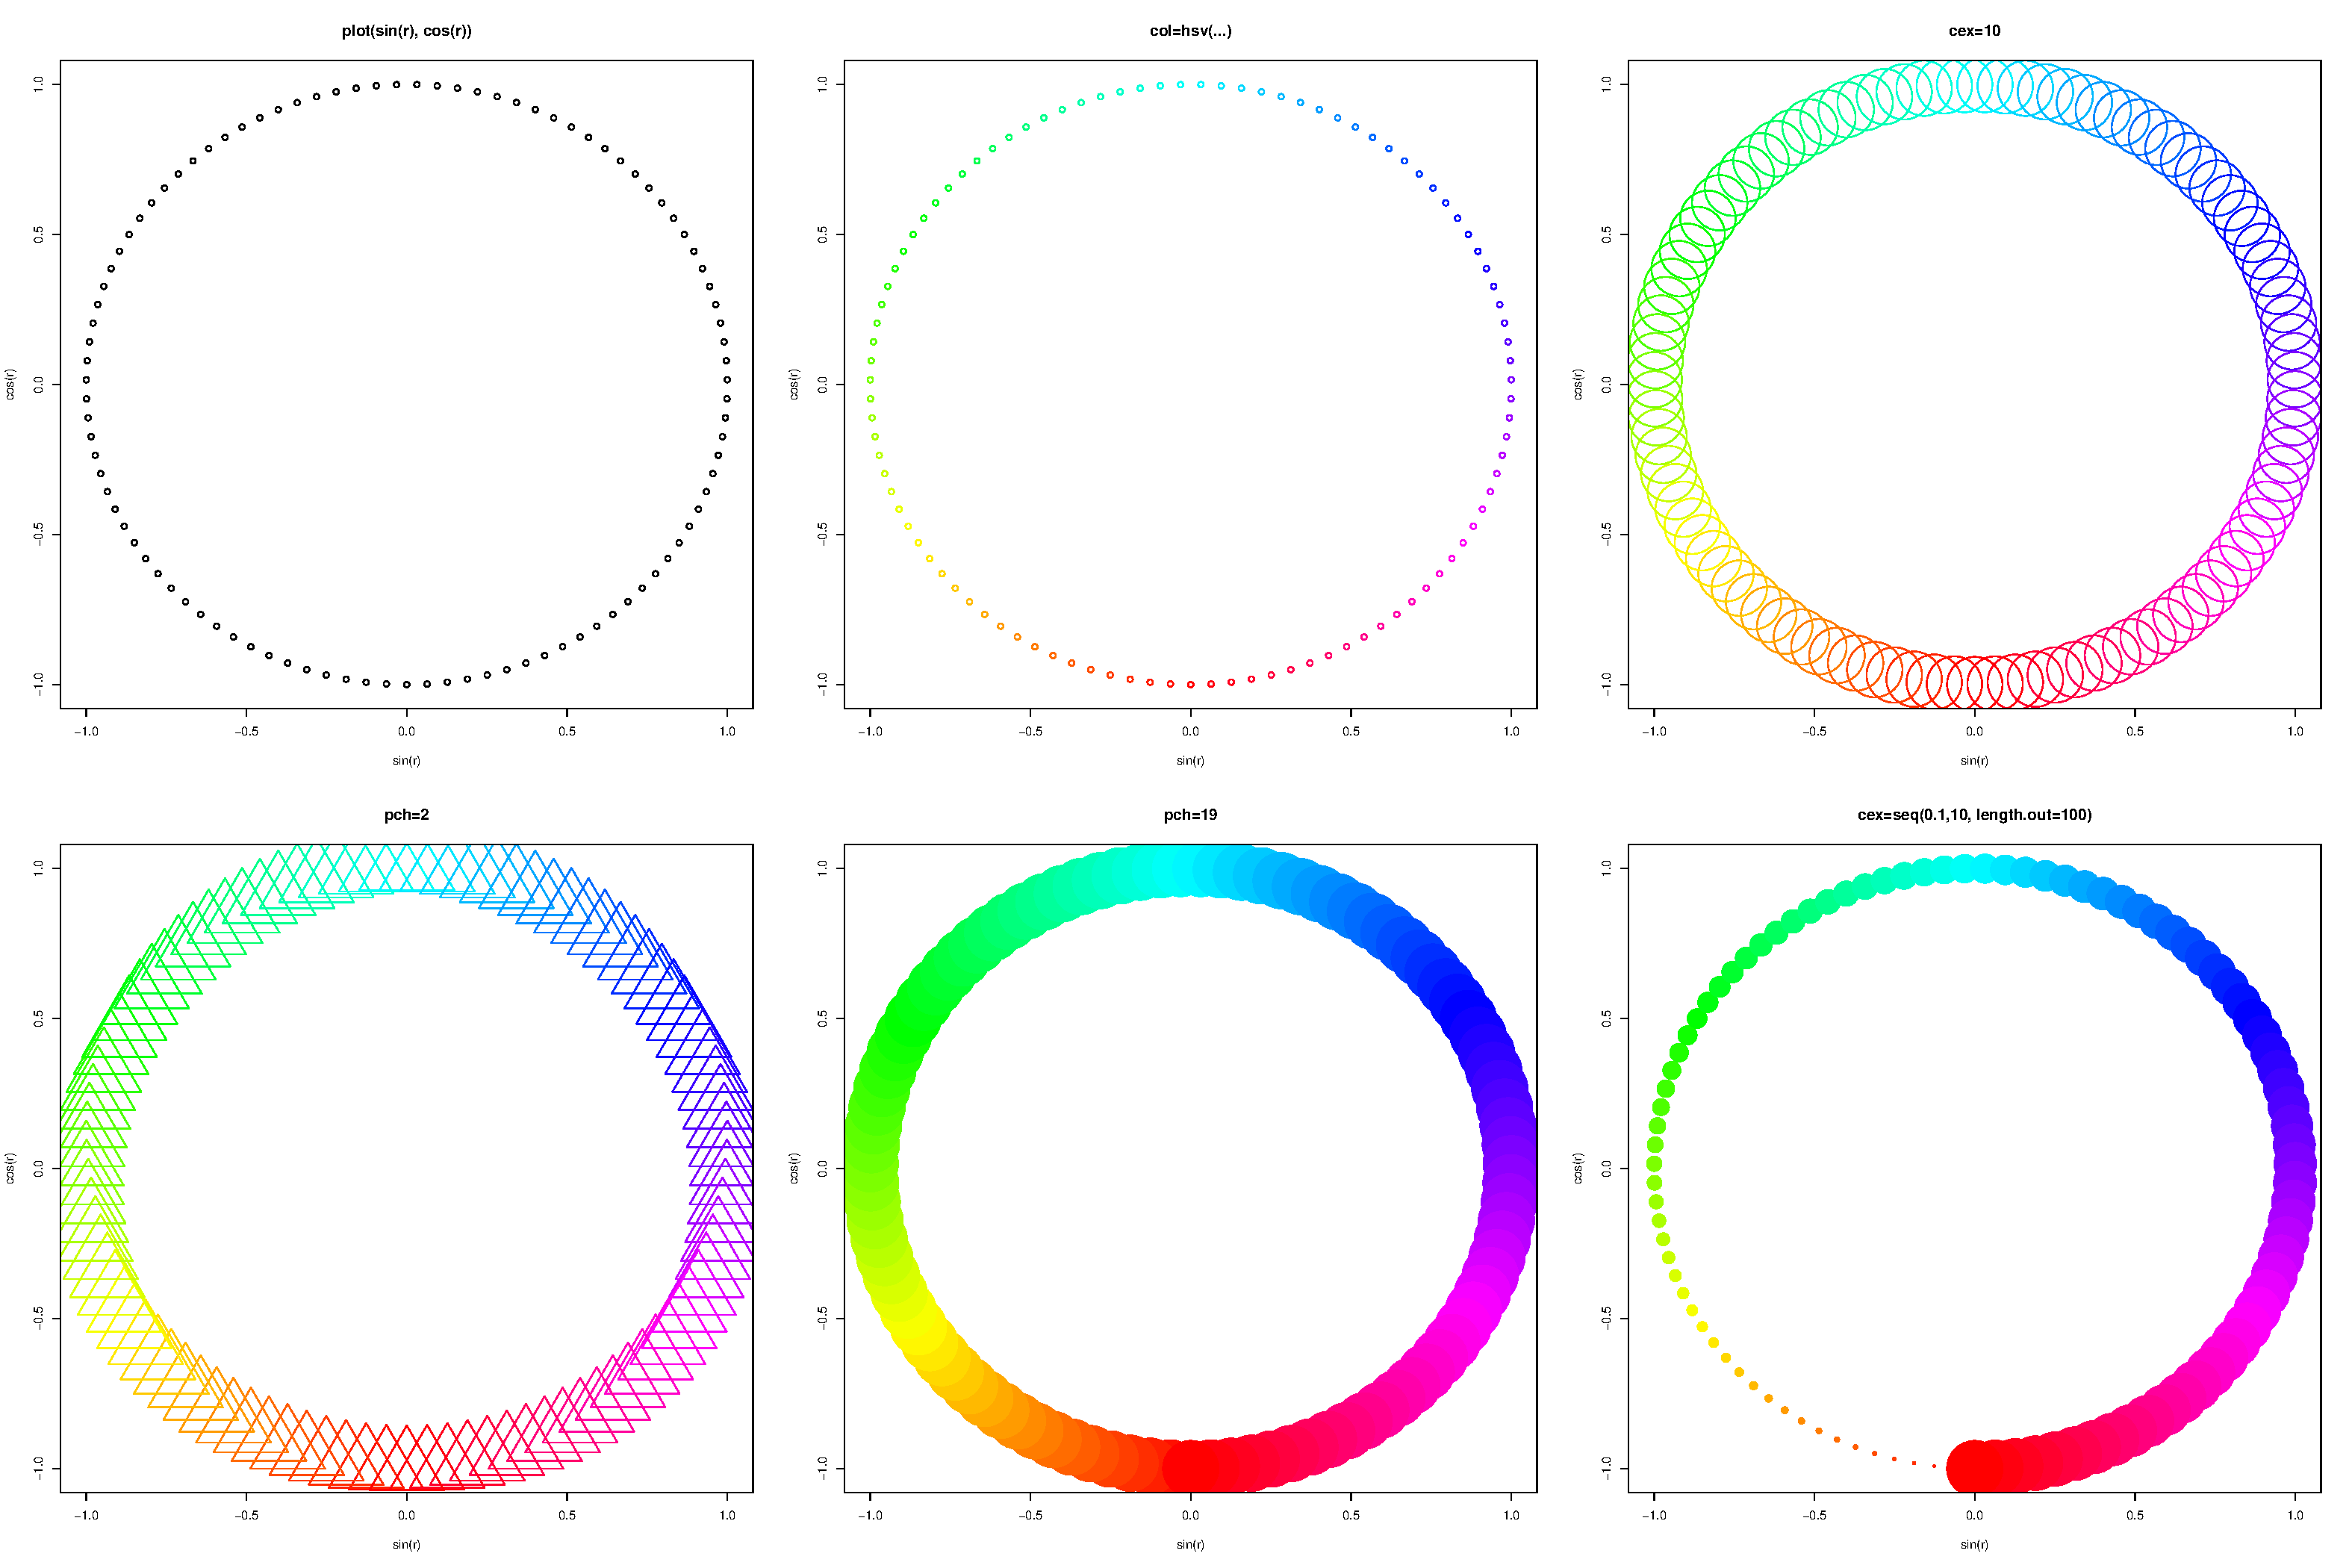
\includegraphics[width=0.7\textwidth]{images/circles.pdf}
  \end{figure}
  \begin{rcode}
    > r <- seq(-pi, +pi, length.out=100)
    par(mfrow=c(2, 3))
    > plot(sin(r), cos(r))
    > plot(sin(r), cos(r), col=hsv(seq(0, 1, length.out=100), 1, 1), cex=1)                            
    > plot(sin(r), cos(r), col=hsv(seq(0, 1, length.out=100), 1, 1), cex=10)
    > plot(sin(r), cos(r), col=hsv(seq(0, 1, length.out=100), 1, 1), cex=10, pch=2)
    > plot(sin(r), cos(r), col=hsv(seq(0, 1, length.out=100), 1, 1), cex=10, pch=19)
  \end{rcode}
\end{frame}

\begin{frame}[fragile]{a spiral}
  \begin{figure}[ht]
    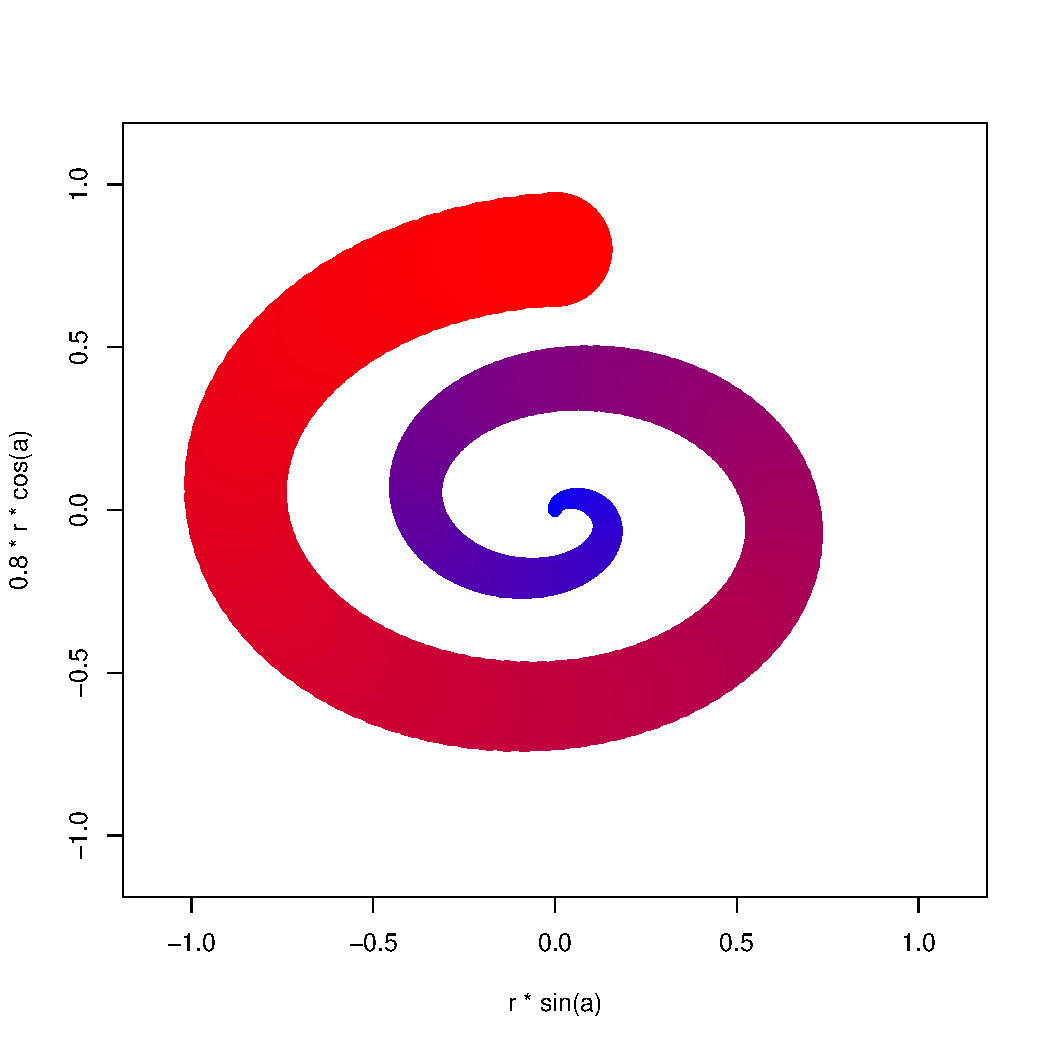
\includegraphics[width=0.5\textwidth]{images/spiral}
  \end{figure}
  \begin{rcode}
    l <- 200
    a <- seq(-2*pi, +2*pi, length.out=l)
    r <- seq(0, 1, length.out=l)
    plot(r*sin(a), 0.8*r*cos(a), pch=19, cex=seq(1, 10, length.out=l),
         col=rgb(seq(0,1,length.out=l), 0, seq(1,0,length.out=l)), xlim=c(-1.1,1.1),
         ylim=c(-1.1,1.1) )
  \end{rcode}
  
\end{frame}

\begin{frame}[fragile]{plotting expression}
  \begin{rcode}
    ## exp.data contains expression patterns (genes in rows, samples in
    ## columns)

    ## fstats.dl.o is the order of the f-statistic for drug effect in
    ## the liver samples.

    ## cor calculates correlation coefficients betwen columns
    ## to get correlations between rows we transpose the data.
    ## Here I'm also scaling it which also requires me to
    ## transpose the data first.

    cr <- cor(scale(exp.data[fstats.dl.o[1],]), scale(t(exp.data)))
    cr.o <- order(cr, decreasing=TRUE)

    ## make matrix of the top 10
    exp.cr <- exp.data[ cr.o[1:10], ]
    
    ## and make a couple of plots:
    pdf("expression.pdf", width=14, height=7)
    par(mfrow=c(1,2))   ## one row

    plot(1, 1, xlim=c(1,ncol(exp.cr)), ylim=range(exp.cr), type='n', xlab='sample', 
         ylab='expression', main="Raw values")
    apply(exp.cr, 1, function(x){ lines(1:length(x), x, col='grey')})
    lines(1:ncol(exp.cr), colMeans(exp.cr), lwd=3)
    
    exp.cr <- t( scale(t(exp.cr)) )
    plot(1, 1, xlim=c(1,ncol(exp.cr)), ylim=range(exp.cr), type='n', xlab='sample', 
         ylab='expression', main="Normalised values")
    apply(exp.cr, 1, function(x){ lines(1:length(x), x, col='grey')})
    lines(1:ncol(exp.cr), colMeans(exp.cr), lwd=3)
    dev.off()
  \end{rcode}
\end{frame}

\begin{frame}{expression plotted}
  \begin{figure}[ht]
    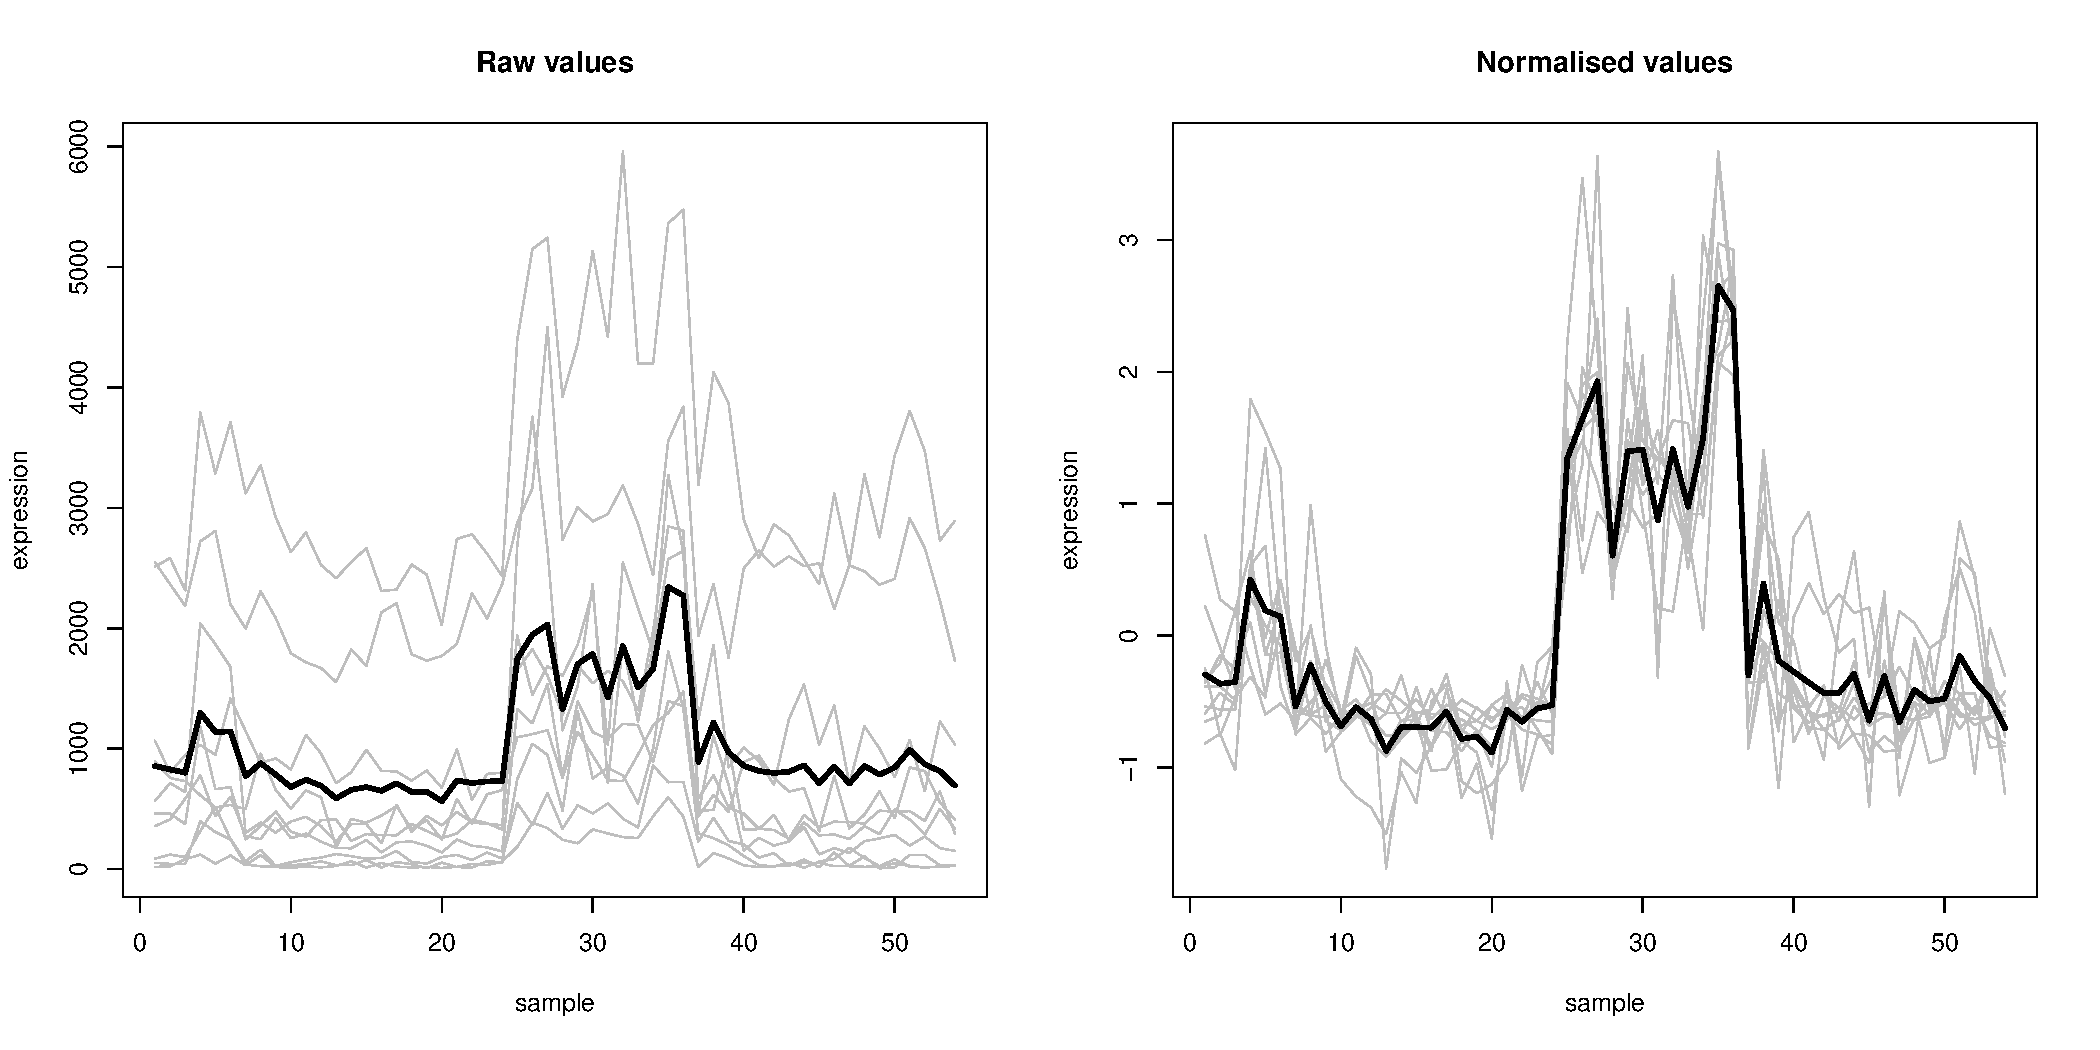
\includegraphics[width=\textwidth]{images/expression}
  \end{figure}
\end{frame}

\begin{frame}[fragile]{arbitrary drawing}
  use rectangles, lines and segments.
  
  \begin{rcode}
    pdf("arbitrary.pdf", width=7, height=7)
    plot(1,1, type='n', axes=FALSE, xlim=c(0,100), ylim=c(0,100), xlab='', ylab='')
    x <- sort(rnorm(40, mean=40, sd=15))
    y <- sort(rnorm(40, mean=50, sd=30))
    r <- abs(rnorm(40, sd=4))
    points(x, y)
    p1 <- sample(1:40, 10)
    p2 <- sample(1:40, 10)
    points(x[p1], y[p2], pch=1:10, cex=2*r[1:10], 
           col=rgb(0,0,1,seq(0.3, 1.0, length.out=10)), lwd=4 )
    
    ## draw some rectangles:
    rect(c(10, 30, 40), c(3, 40, 80), c(15, 40, 47), c(12, 43, 82), lwd=c(1,2,3),
         col=c('grey', rgb(0.3, 0, 0.8, 0.5), hsv(0.3, 0.5, 0.8, 0.3)) )

    ## draw a filled ellipse
    a <- seq(-pi,pi, length.out=100)
    polygon(50+20*sin(a), 50+40*cos(a), col=rgb(0, 0.5, 0.5, 0.8), border='green') 
    
    ## a bit of text
    text(c(10, 10), c(60, 50), labels=c('hello', 'there'), cex=3)
    dev.off()
  \end{rcode}
  
  \huge $\Rightarrow$
\end{frame}

\begin{frame}{drawn arbitrarily}
  \begin{figure}[ht]
    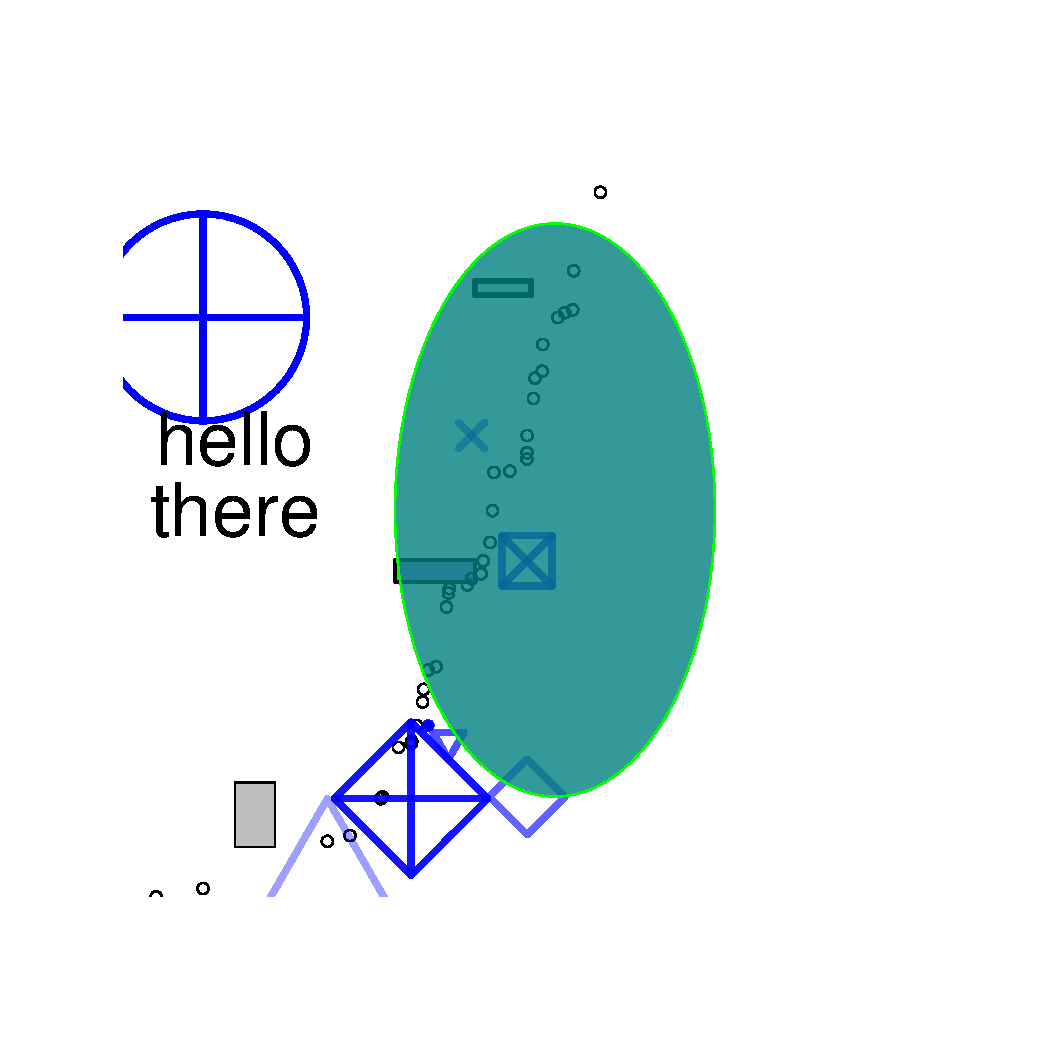
\includegraphics[width=0.8\textwidth]{R/arbitrary}
  \end{figure}
\end{frame}


\begin{frame}{A Smith Waterman matrix}
  \begin{figure}[ht]
    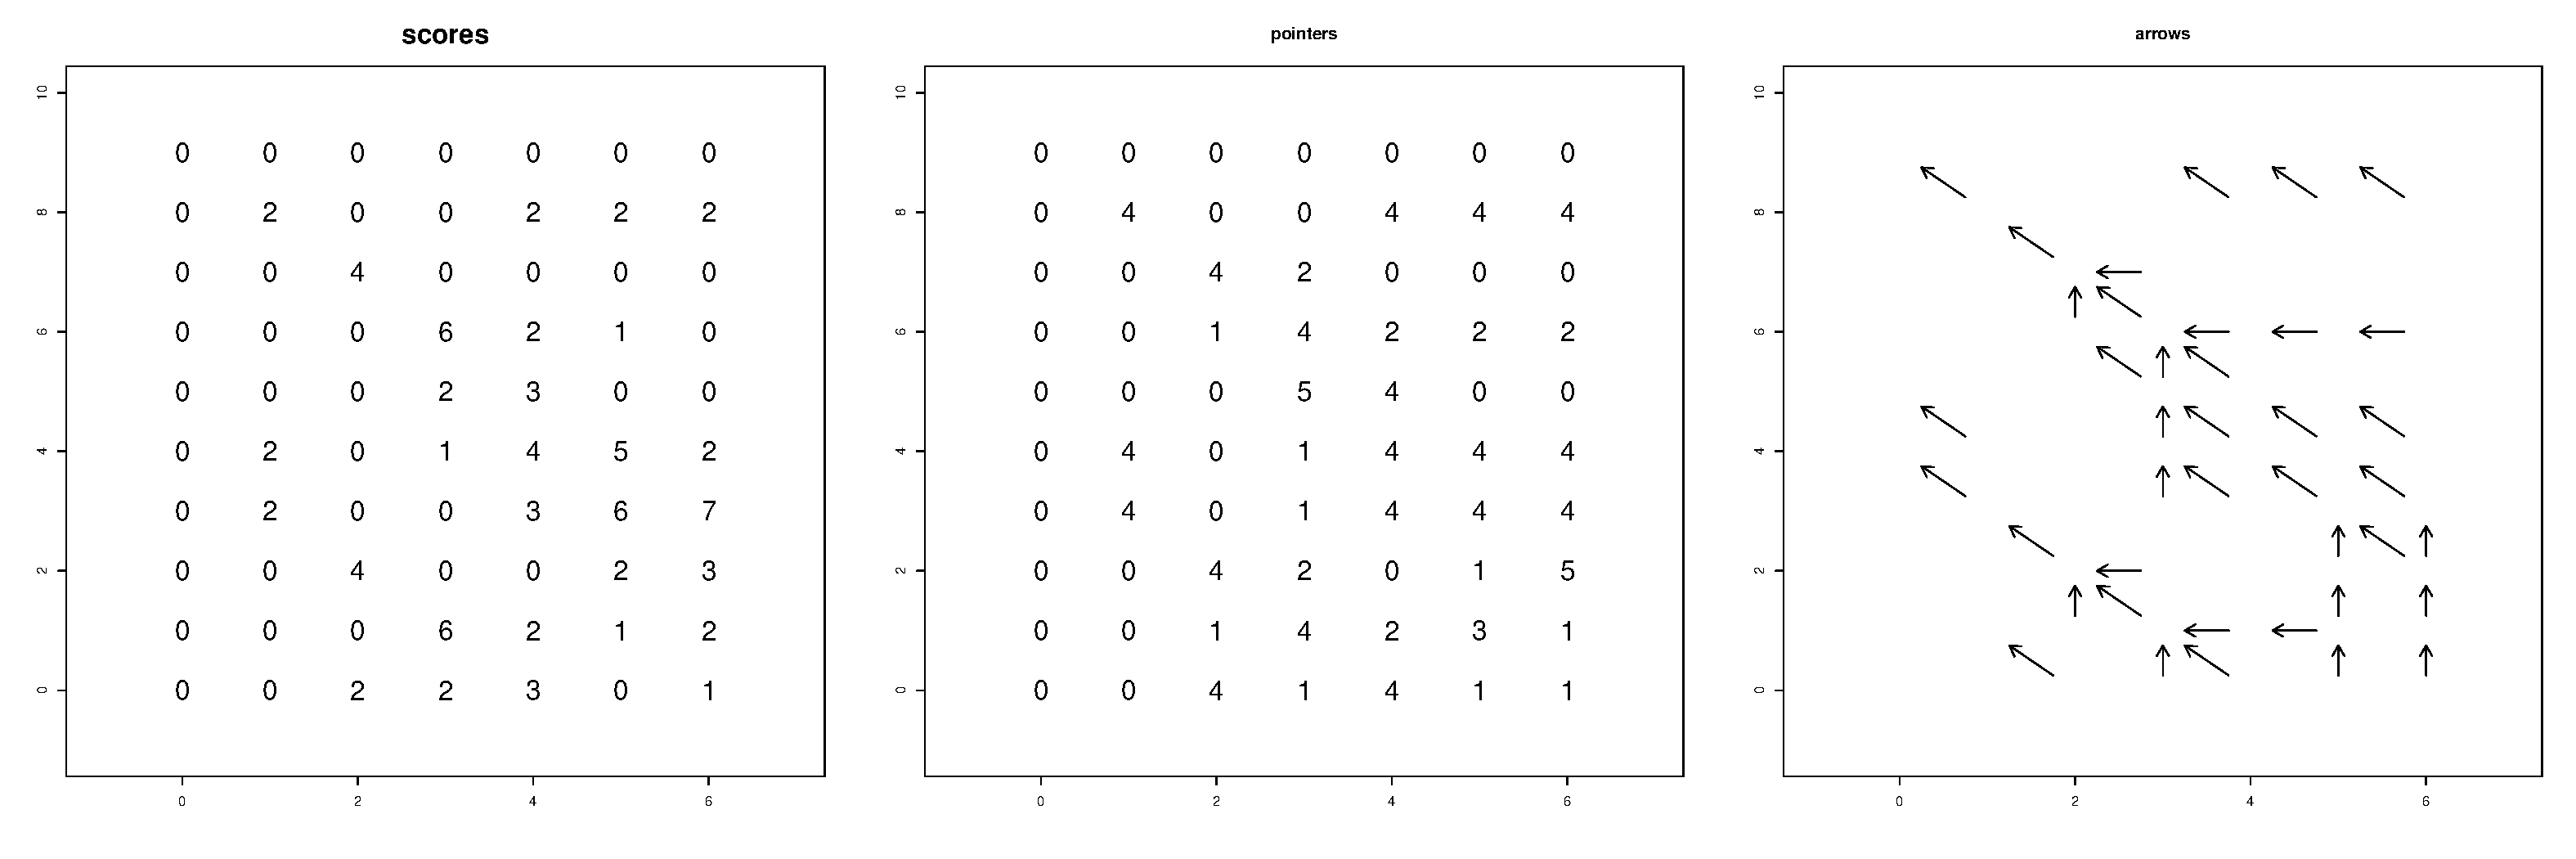
\includegraphics[width=\textwidth]{R/SM_drawing}
  \end{figure}
\end{frame}


\begin{frame}[fragile]{drawing a Smith Waterman matrix}
  \begin{rcode}
    scores <- as.matrix(read.table('SM_scores'))
    ptrs <- as.matrix(read.table('SM_pointers'))
    
    ## to draw them first set up a set of positions                                                                          
    
    x <- as.integer( 0:(length(ptrs)-1) / nrow(ptrs) )
    y <- ( 0:(length(ptrs)-1) %% nrow(ptrs) )
    y <- max(y) - y
    
    pdf(``SM_drawing.pdf'', width=21, height=7)
    par(mfrow=c(1,3))
    plot( 1, xlim=c(-1, max(x)+1), ylim=c(-1, max(y)+1),
    type='n', xlab='', ylab='', main='scores', cex.main=2 )
    text(x, y, labels=as.numeric(scores), cex=2)
    
    plot( 1, xlim=c(-1, max(x)+1), ylim=c(-1, max(y)+1),
    type='n', xlab='', ylab='', main='pointers', cex.main=2 )
    text(x, y, labels=as.numeric(ptrs), cex=2) 
    
    plot( 1, xlim=c(-1, max(x)+1), ylim=c(-1, max(y)+1),
    type='n', xlab='', ylab='', main='arrows',cex.main=2 )
    up.b <- as.logical(bitwAnd(1, ptrs))
    left.b <- as.logical(bitwAnd(2, ptrs))
    diag.b <- as.logical(bitwAnd(4, ptrs))
    arrows( x[up.b], y[up.b]+0.25, x[up.b], y[up.b] + 0.75, length=0.1 )
    arrows( x[left.b]-0.25, y[left.b], x[left.b] -0.75, y[left.b], length=0.1 )
    arrows( x[diag.b]-0.25, y[diag.b]+0.25, x[diag.b] -0.75 , y[diag.b] + 0.75,
    length=0.1 )
    dev.off()
  \end{rcode}
\end{frame}

\begin{frame}{Visualising unstructured data}
  \begin{figure}[ht]
    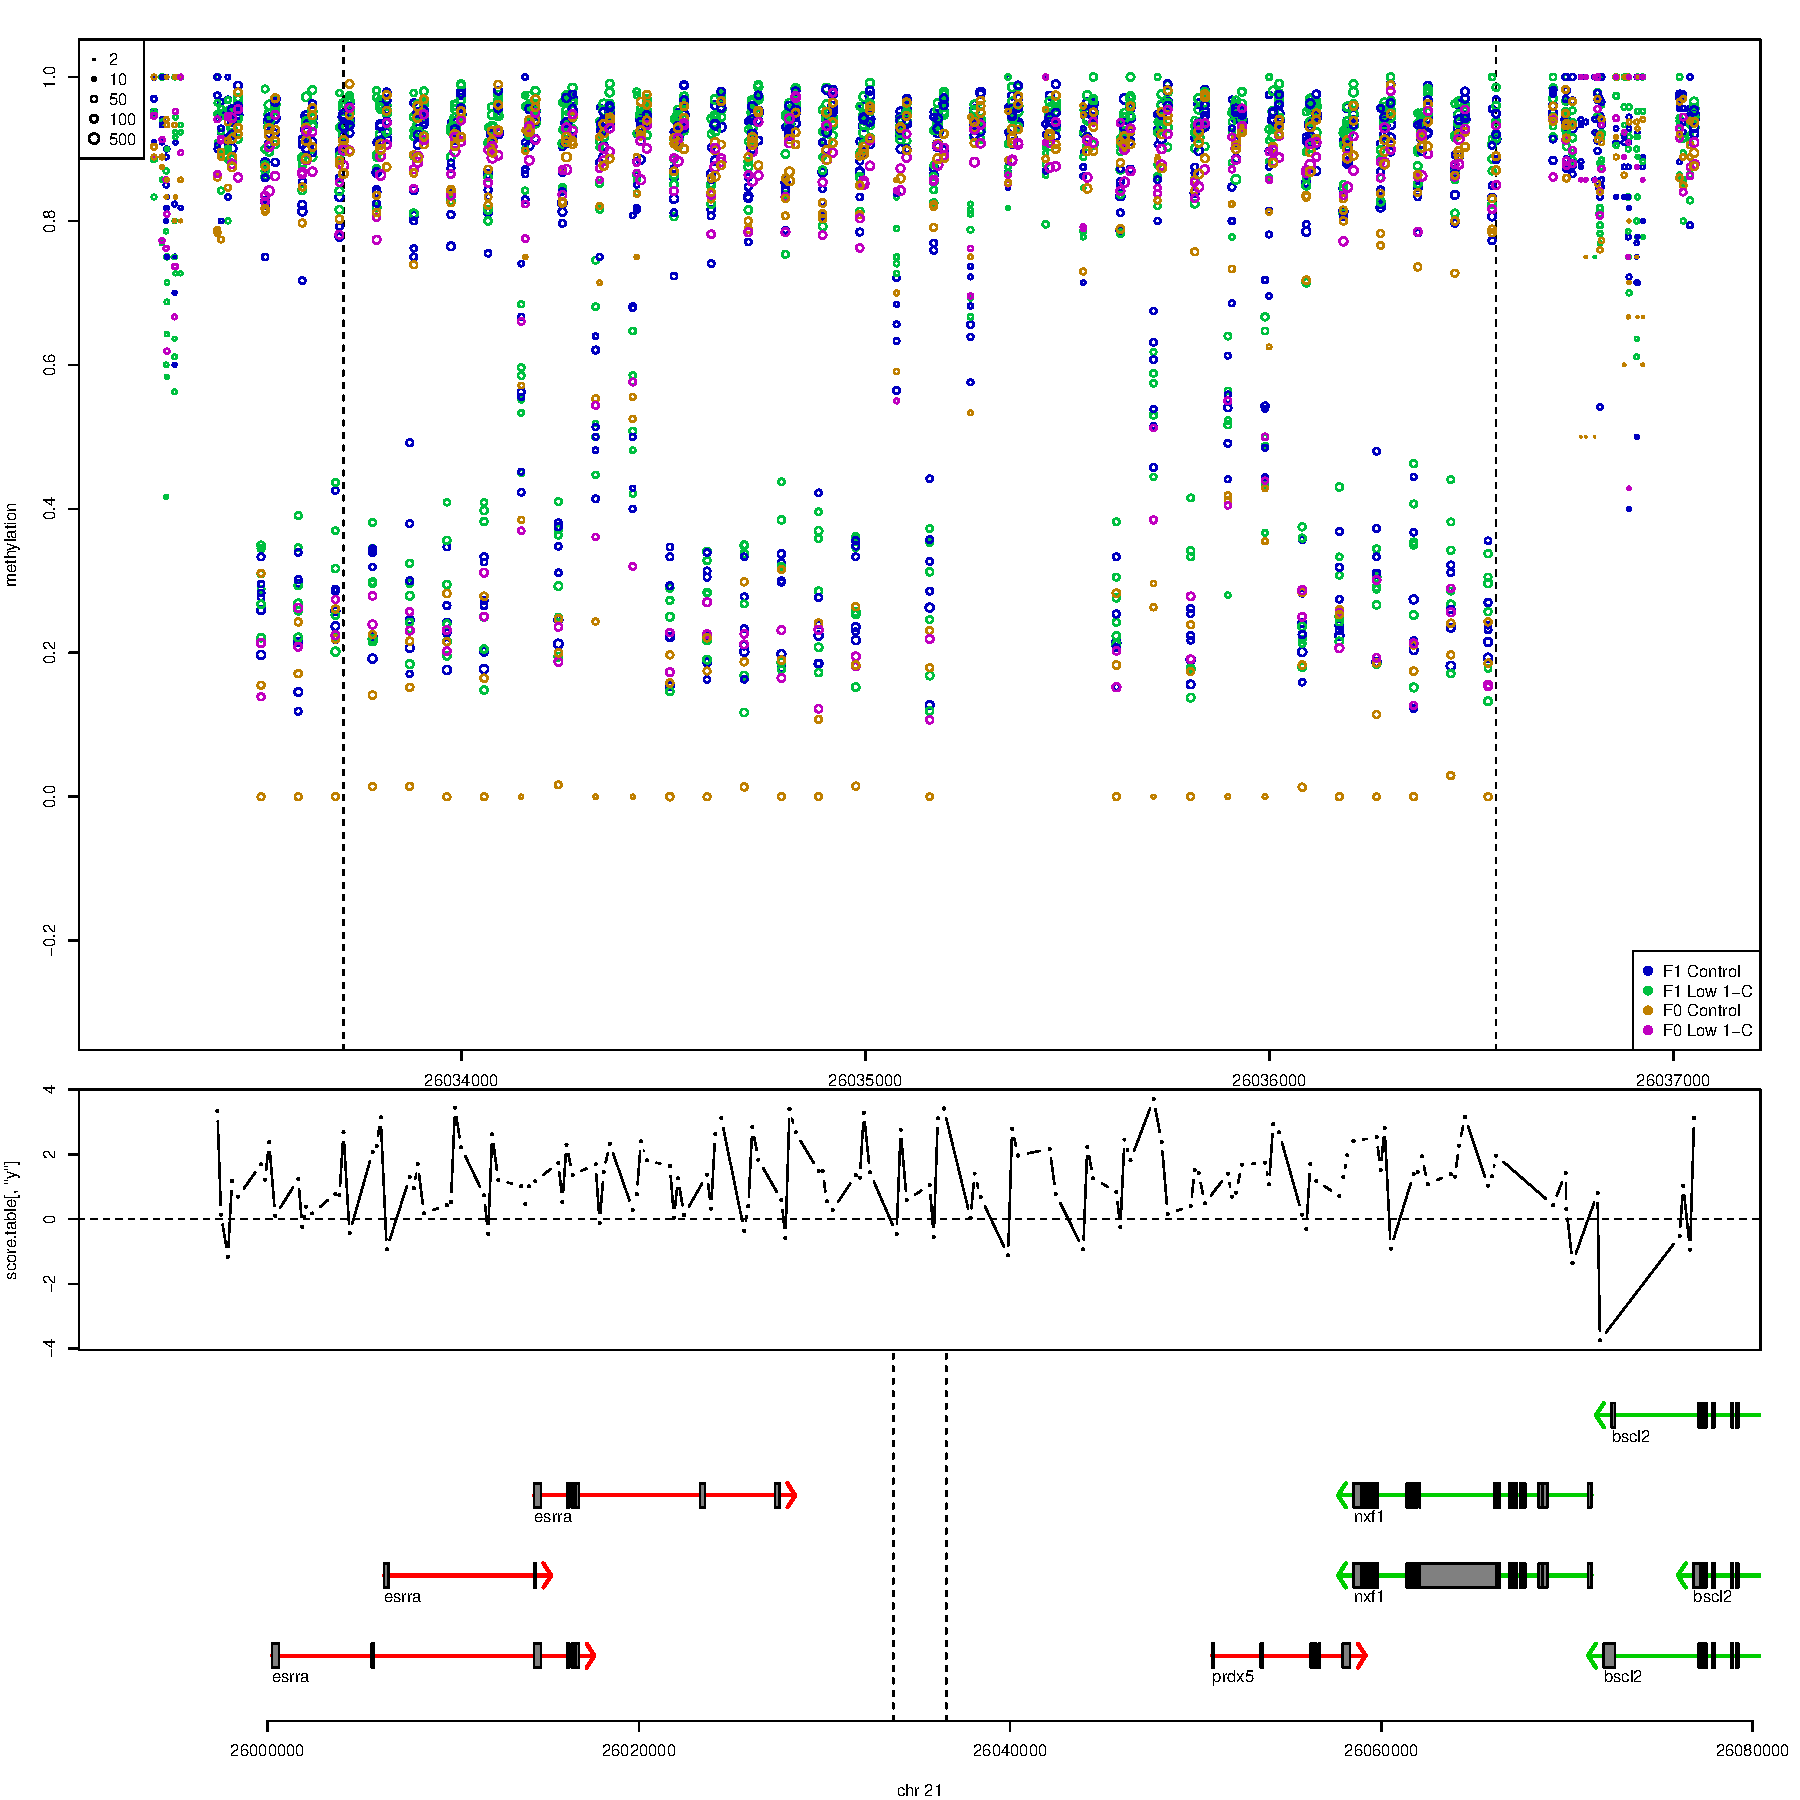
\includegraphics[width=0.78\textwidth]{images/genome_plot.pdf}
  \end{figure}
  
\end{frame}

\begin{frame}[fragile]{defining functions}
  You should always avoid doing the same thing more than once;

  functions are one way to reuse code. In R they are treated
  as objects that can easily be passed to other functions
  (eg. as in \texttt{apply}).

  \begin{rcode}
    ## to define a function use the function function...
    myFunction <- function(a, b){
      ## the last statement is just returned
      a * b
    }
    ## use the function
    > myFunction(2,3)
    [1] 6

    ## and hey it's vectorised as its underlying operations are
    > myFunction(1:10, 1:10)
    [1]   1   4   9  16  25  36  49  64  81 100
  \end{rcode}

  use\\
  \hspace{4em} \verb|function(arguments){ function body }|

  to define new functions
\end{frame}

\begin{frame}{other stuff}
  \begin{itemize}
  \item \texttt{par()}. This sets plotting parameters. There are
    a very large number around, see, \texttt{?par} for further details.
  \item \texttt{image} Plots the values in a matrix, mapping values to
    colours. The basis for heatmaps of various sorts.
  \item \texttt{identify} Lets you identify and label items on a plot
    in an interactive manner.
 \end{itemize}
 
 Remember that you can always decorate a plot arbitrarily after it's
 been plotted by some higher level fuction. To get the coordinates that
 have been plotted use: \texttt{par("usr")}

\end{frame}

\begin{frame}[fragile]{function arguments}
  The arguments to your new function are specified as arguments
  to the \texttt{function()} function.

  Defaults can be specified for each argument. Which will be used
  if not specifed:

  \begin{rcode}
    myFunction <- function(a=10, b=5){
      a * b
    }
    
    > myFunction(10, 10)
    [1] 100

    > myFunction(3)  ## a will take the argument
    [1] 15

    > myFunction()
    [1] 50

    ## you can make use of the names
    > myFunction(b=20)
    [1] 200
  \end{rcode}
\end{frame}

\begin{frame}[fragile]{the ellipsis}
  in R, the ellipsis, (\texttt{...}) is often used to
  pass arguments from one function to nested functions.

  For example you may wish to make a special plot function
  
  \begin{rcode}
    cubePlot <- function(x, ...){
      ## your function plots the cube of values
      plot(x, x^3, ...)
    }
    ## this allows the user to specify arguments that will
    ## be sent to the plot function:
    pdf("cubeplot.pdf", width=14, height=7)
    par(mfrow=c(1,2))
    cubePlot(-10:10)
    cubePlot(-10:10, main='cubes of -10 to +10', xlab='x', ylab='y', type='b')
    dev.off()
  \end{rcode}

  \huge $\Rightarrow$
\end{frame}

\begin{frame}{cubePlot}
  \begin{figure}[ht]
    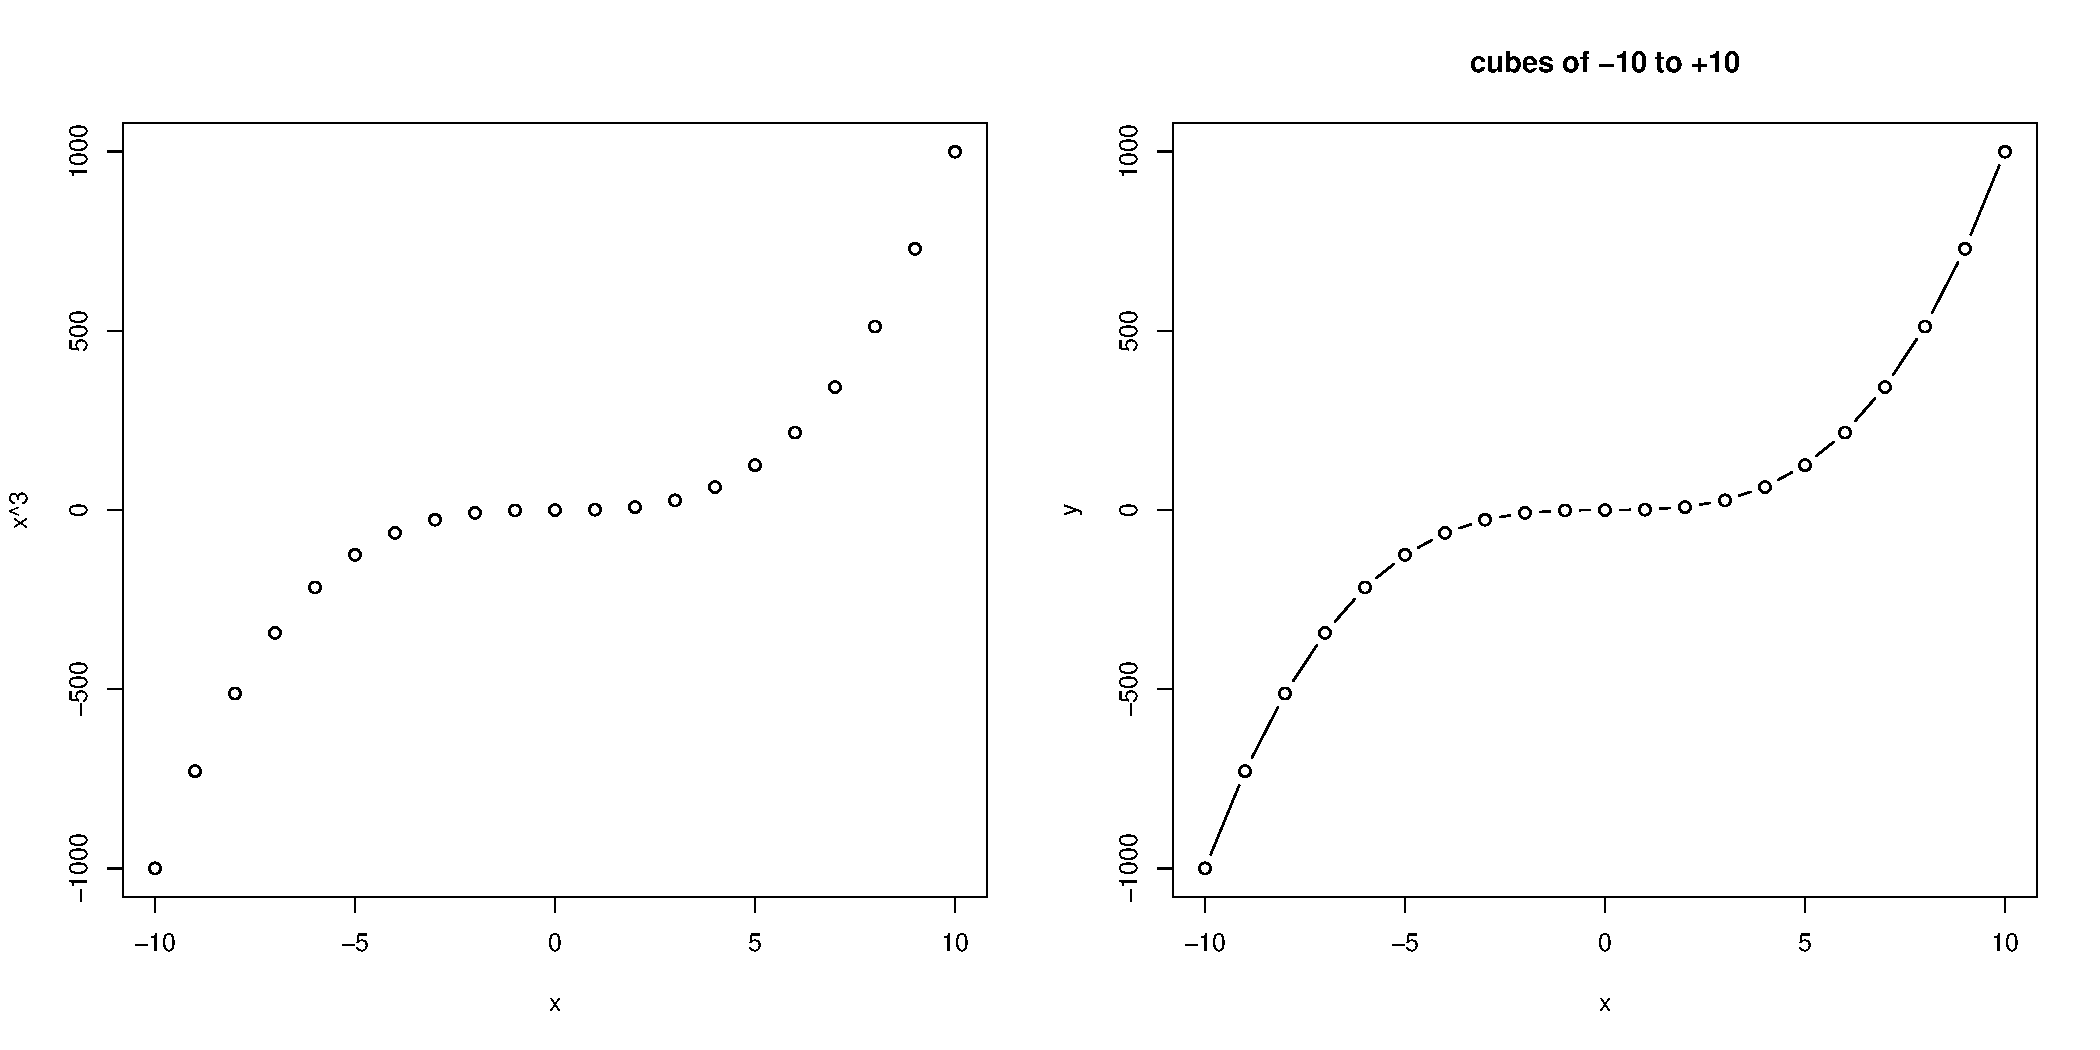
\includegraphics[width=\textwidth]{images/cubeplot.pdf}
  \end{figure}

  The result of \texttt{cubePlot()} without and with arguments
  fed forward using \texttt{...}
\end{frame}

\begin{frame}{classes in R}
  Classes are complicated in R. There are at least three different types.

  \begin{itemize}
  \item S3 classes. The simplest kind of class.
  \item S4 classes. Newer class that has methods and slots.
  \item Reference classes. These don't seem to have a specific names.
    They can be passed by reference in functions and behave quite differently
    to other objects in R.
  \end{itemize}
  
  to understand these, check out Hadley's pages linked above.
\end{frame}

\begin{frame}{The most important R function}

\texttt{?}

learn to read the manual pages!

don't just read, but experiment with the functions, arguments, options
and numbers to work out what is going on.
\end{frame}

\end{document}
